\chapter{معامله گر خودکار}
\section{مقدمه}
\par
با ظهور و گسترش الگوریتم های مختلف هوش مصنوعی به تدریج این فناوری ها جای خود را در دنیای اقتصاد هم باز کردند . سیستم های معامله گر خودکار نوعی از نرم افزار ها هستند که طبق برخی از قوانینی که معامله گران برای آن ها تعریف کرده اند به صورت خودکار بر اساس اطلاعات مختلف معاملاتی را در بازار های مختلف مانند بورس و یا ارز های دیجیتال انجام می دهند . 

گزارش داده شده است که در حدود 75 درصد از معاملات بورس آمریکا توسط همین سیستم های خودکار معاملات انجام می پذیرد
\cite{chan2021quantitative}
.
\begin{figure}[h]
	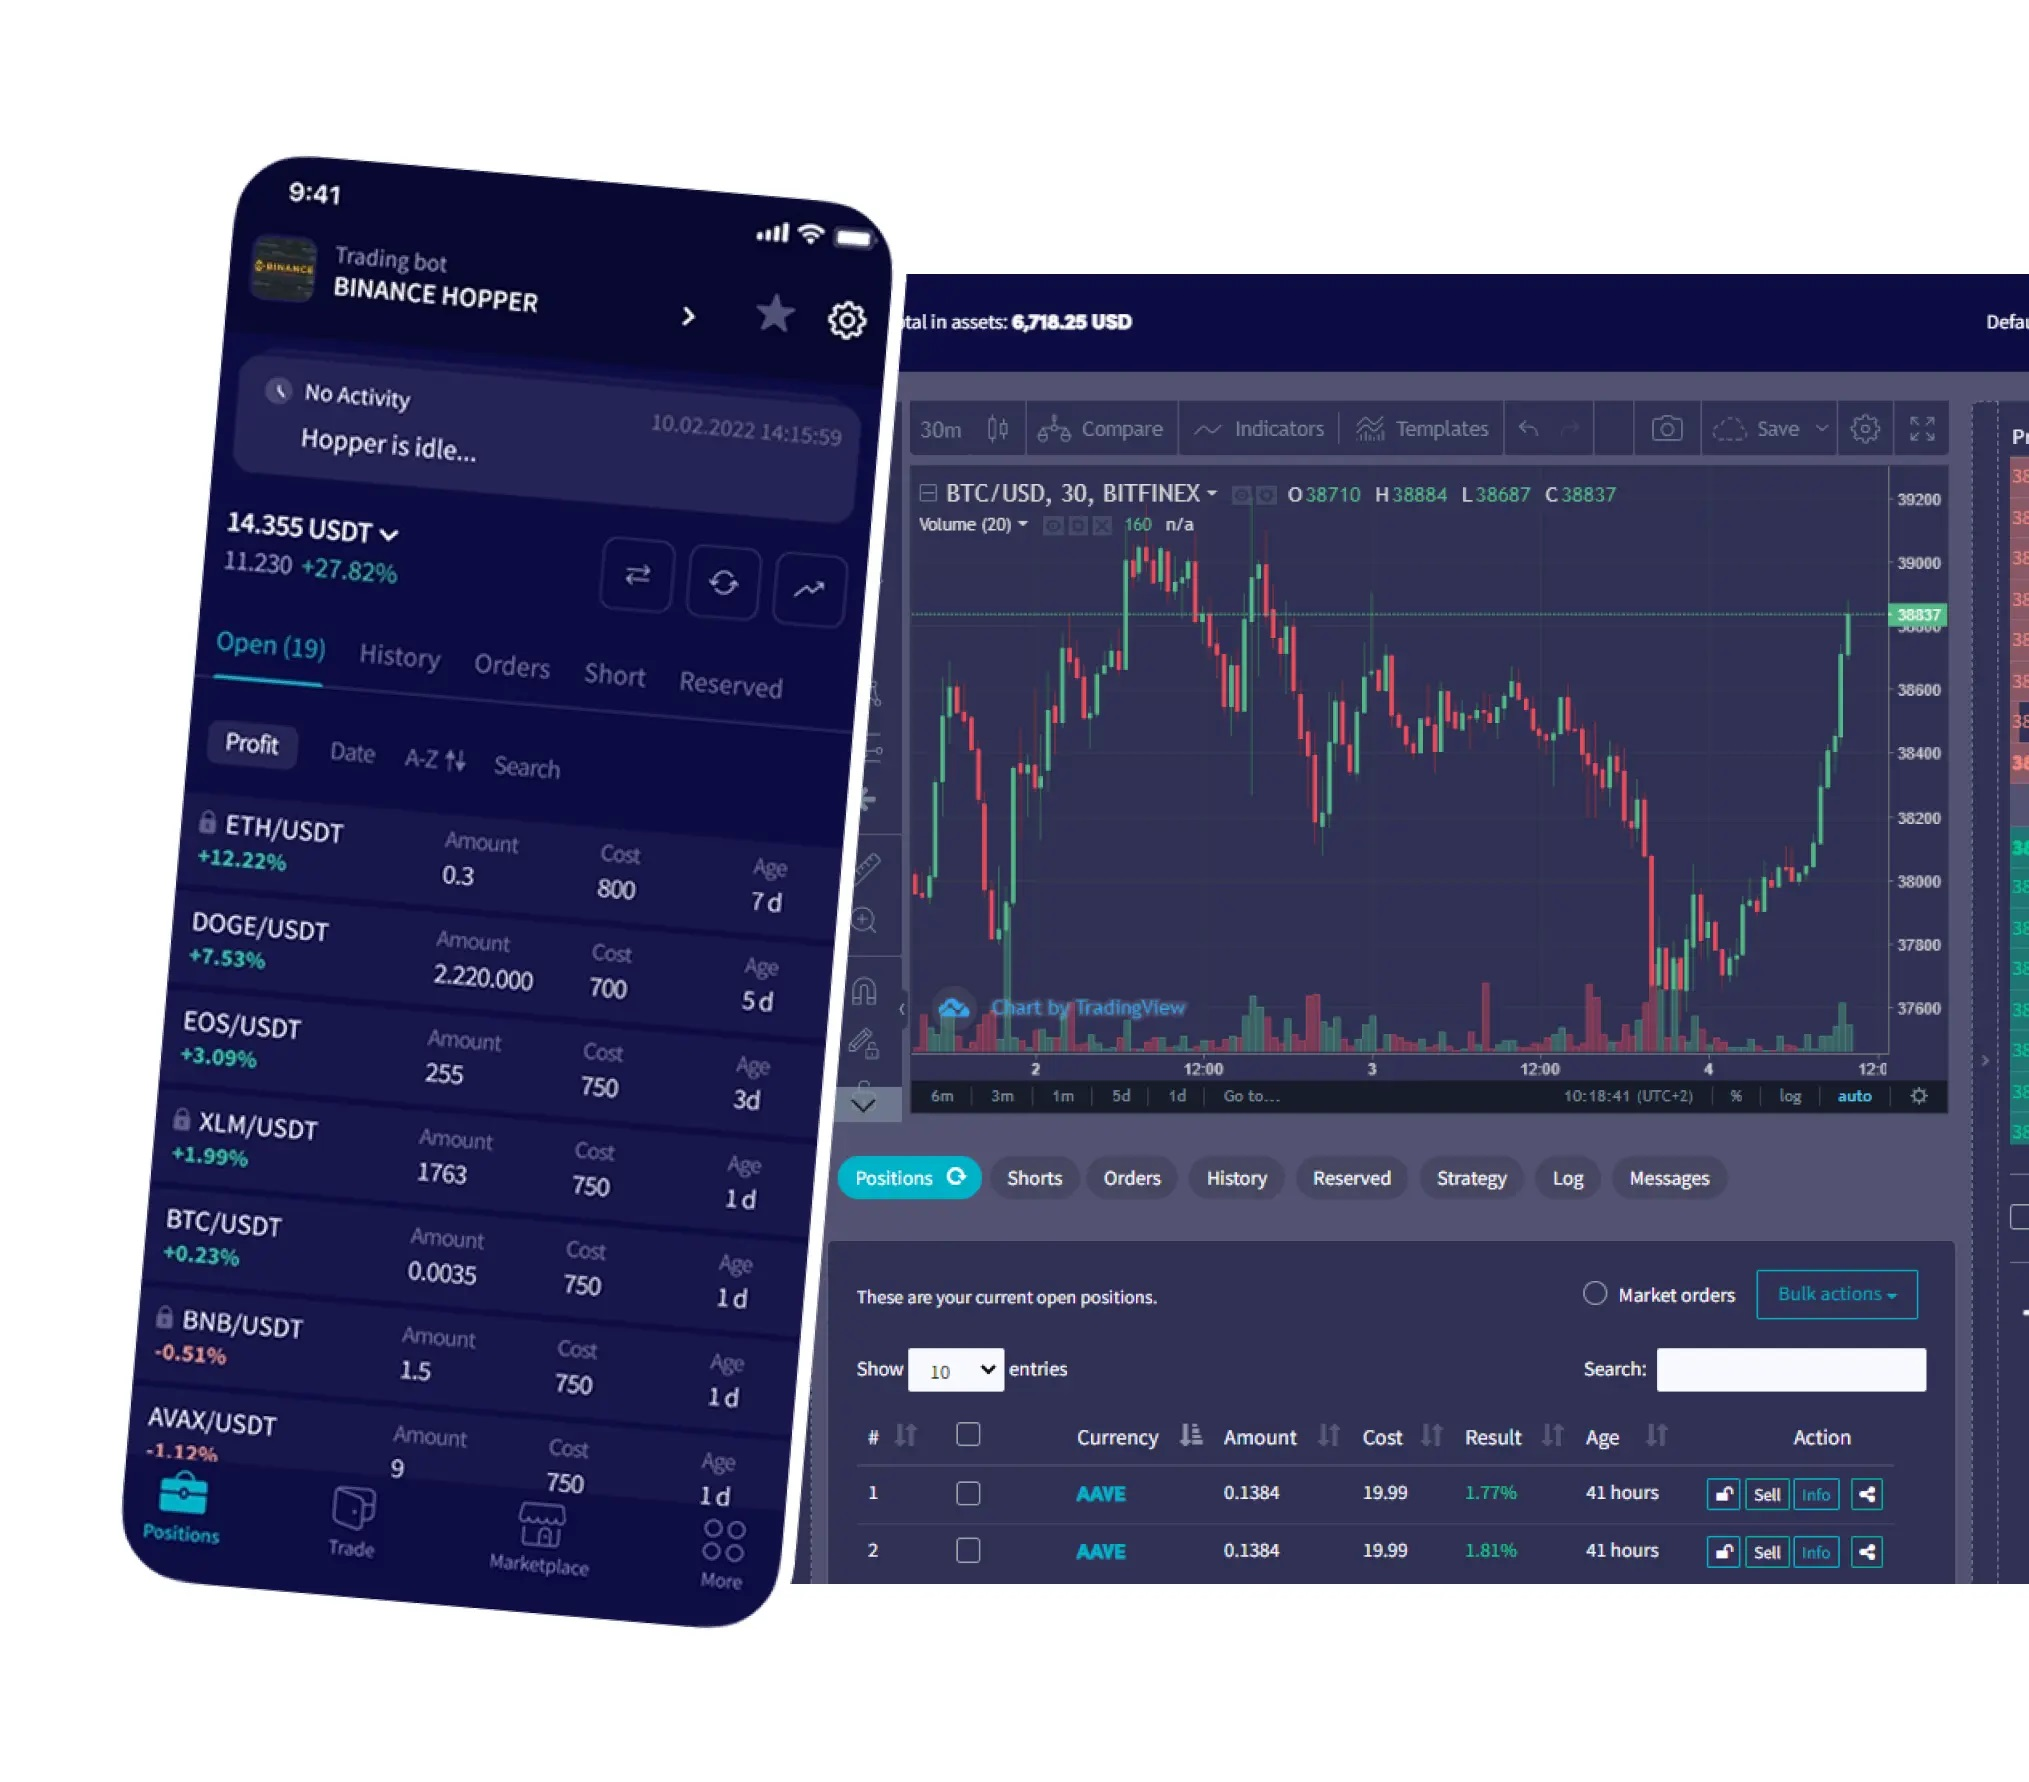
\includegraphics[scale=0.2]{trade}
	\centering
	\caption{ربات  معاملات خودکار برای  بازار ارز های دیجیتال}
	\cite{cryptohopper}
	\label{trade:fig1}
\end{figure} 
\section{طرح مسئله}
در
\cite{tran2023optimizing}
به سیستم های معامله گر خودکار برای بازار ارزهای دیجیتال بر اساس یادگیری تقویتی اشاره شده است . یک سیستم که بتواند بدون دخالت انسان و به صورت خودمختار با توجه به داده های بازار معاملاتی را انجام دهد و با استفاده از یادگیری تقویتی عمیق بیشترین سود را از معاملات بدست آورد .

\section{مدل\lr{PEAS}} 
سیستم های معامله گر خودکار به صورت سامانه هایی هوشمند می توانند تصمیمات مناسب را به دور از هیجاناتی که انسان ها دچار آن می شوند معاملات را طبق قوانین معلوم انجام دهند . در ادامه به بررسی مدل این سیستم ها می کنیم .
\subsection{اندازه گیری عمکرد} 
برای اندازه گیری عملکرد یک چنین سیستم هایی می توان به سود ماهیانه ی آن ها توجه کرد . در 
\cite{tran2023optimizing}
بهترین و بدترین و مقدار متوسط سود ماهیانه به عنوان تابع عملکرد و تابع جایزه یادگیری تقویتی در نظر گرفته شده اند .
\subsection{محیط}
محیط در مورد مسئله ی فوق مجموعه حالت هایی است که سیستم می تواند در آن ها قرار گیرد . حالت این سیستم می تواند با میزان دارایی ها و سرمایه ی سیستم به علاوه ی اطلاعات قیمت کالای معاملاتی - که در این جا ارز دیجیتال است - باشد . 
\par 
محیط به صورت کامل رویت پذیر
\footnote{\lr{fully observable}}
می باشد . محیط دائم در حال تغییر است و بنابراین به صورت پویا
\footnote{\lr{dynamic}}
است . این نکته مهم است که این تغییرات می توانند به صورت تصادفی باشند و گاهی قیمت کالایی نوسان داشته باشد . طبیعتا در بازار کاربران دیگری هم در حال معامله می باشند و محیط به صورت چند کاربره است . 
محیط به صورت 
\lr{episodic}
می باشد و به علت بزرگ بودن بازار رفتار محیط به 
\lr{action}
های 
\lr{agent} 
وابسته نیست . 
هم چنین تغییرات سیستم به صورت گسسته در نظرگرفته شده است .

\subsection{عملگر}
عملیات های سیتم باید توسط برخی از قوانین که برای نرم افزار تعریف شده اند محدود شوند . عملیات های نرم افزار متنوع هستند و می توانند شامل فروش مقداری خاص از نوعی ارز  باشند .
\subsection{حسگر}
به منظور تشخیص وضعیت بازار نیاز است سیستم مستقیم به سایت معاملاتی اتصال داشته باشد و اطلاعات مورد نیاز خود از محیط را به صورت سیگنال هایی از آن دریافت نماید .
\section{جمع بندی}
در فصل فعلی به بررسی کلی از سامانه  های معامله گر پرداختیم و به صورت کلی به شیوه ی عملکرد آن ها پرداختیم . هر یک از عملیات هایی که ربات معامله گر انجام می دهند با توجه به 
\lr{rationality}
است و سعی دارد تا پاسخ مناسب بدهند وتابع سود را بیشینه کند .





